\documentclass{article}
\usepackage{microtype}
\usepackage{amsmath}
\usepackage{graphicx}
\usepackage{subfigure}
\usepackage{booktabs}
\usepackage{multirow}
\usepackage{hyperref}
\newcommand{\theHalgorithm}{\arabic{algorithm}}
\usepackage[accepted]{icml2021}
\usepackage[T1]{fontenc}
\hypersetup{hypertexnames=false}
\makeatletter\let\tableinput\@@input\makeatother
\makeatletter
\renewcommand{\Notice@String}{Interim course project report. Not a conference publication.}
\makeatother
\icmltitlerunning{Joint-angle features for static ASL fingerspelling}
\begin{document}
\appendix
\onecolumn
\setcounter{figure}{2}
\setcounter{table}{2}
\section{Complete Letter-Level Results}\label{app:letters}
Table~\ref{tab:letters} includes every letter, not only selected gains or regressions. Metrics are percentages; $\Delta n$ is the change in correct true-letter images. ``Base'' is the project-profile SVM with 820 Shin inputs; ``Angles'' adds the 15 continuous measurements. Support varies because detection filtering is not uniform across letters. Precision measures the correctness of predictions of a letter, while recall measures recovery of its true images.
\begin{table}[h]\centering\caption{All-letter pooled OOF comparison.}\label{tab:letters}
\begin{tabular}{lrrrrrrrr}\toprule
 & & \multicolumn{2}{c}{Precision (\%)} & \multicolumn{2}{c}{Recall (\%)} & \multicolumn{2}{c}{F1 (\%)} & \\
Letter & Images & Base & Angles & Base & Angles & Base & Angles & $\Delta n$\\\midrule
\tableinput letter_rows.tex 
\bottomrule\end{tabular}\end{table}

The remaining angle-model errors include R$\rightarrow$U (142), N$\rightarrow$M (141), M$\rightarrow$N (102), U$\rightarrow$R (44), D$\rightarrow$O (41), Q$\rightarrow$P (41) and O$\rightarrow$D (19). These counts suggest several candidate investigations; prioritizing only D/O would ignore larger residual error sources. Full ordered error pairs are retained in \texttt{results/angles/confusions/all\_error\_pairs.csv}.

\clearpage
\section{Full Confusion Matrices}
\begin{figure}[h]\centering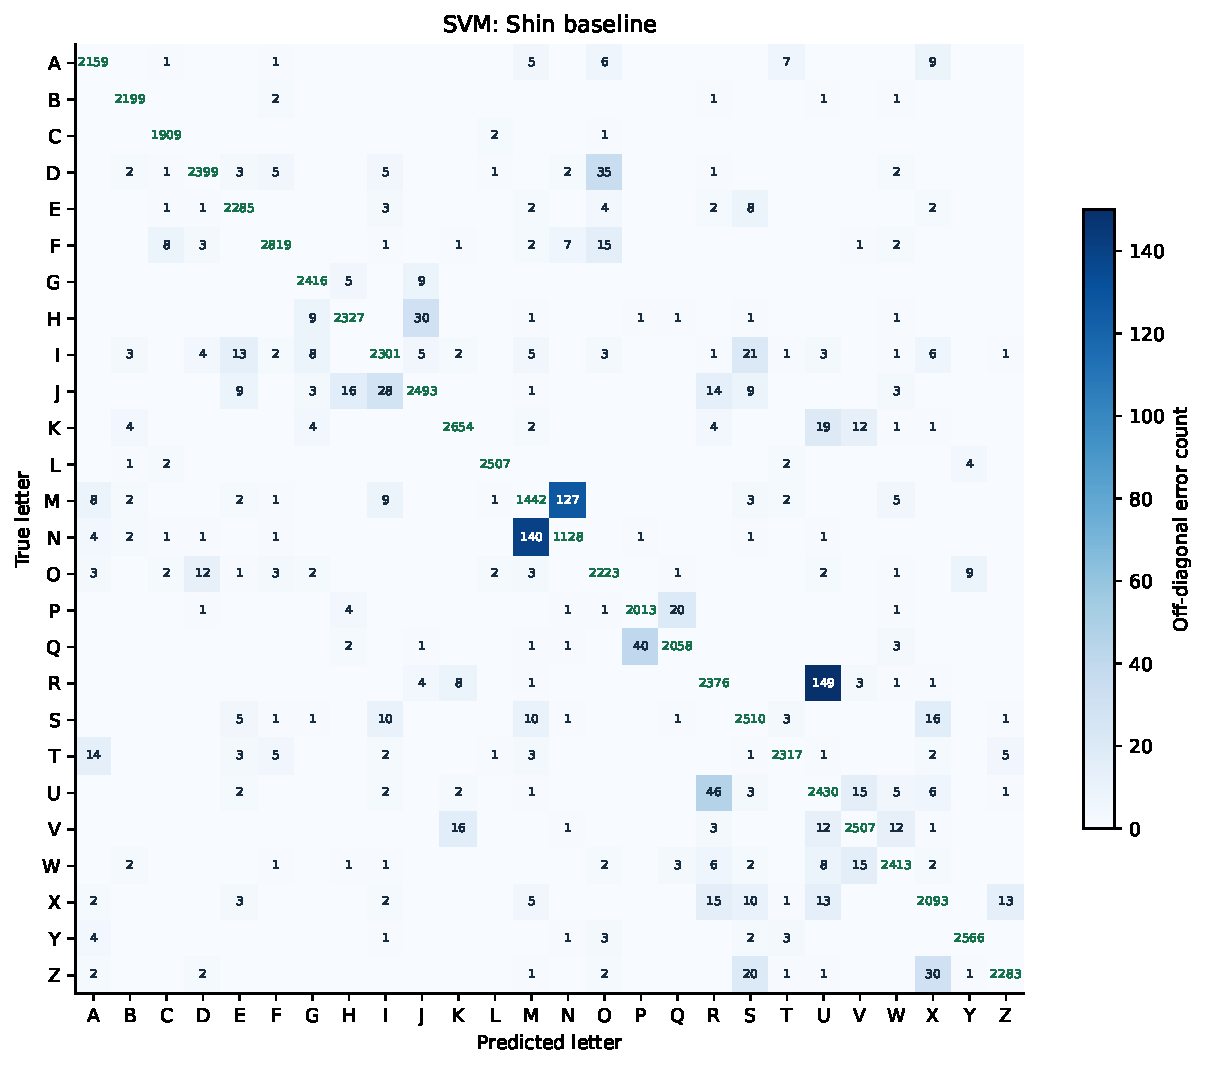
\includegraphics[width=.91\linewidth]{figures/confusion_shin.pdf}
\caption{SVM baseline OOF confusion counts for all 26 letters. Diagonal counts are green; shading is restricted to off-diagonal errors to keep smaller confusions visible. Rows are true labels and columns predictions.}\end{figure}
\clearpage
\begin{figure}[h]\centering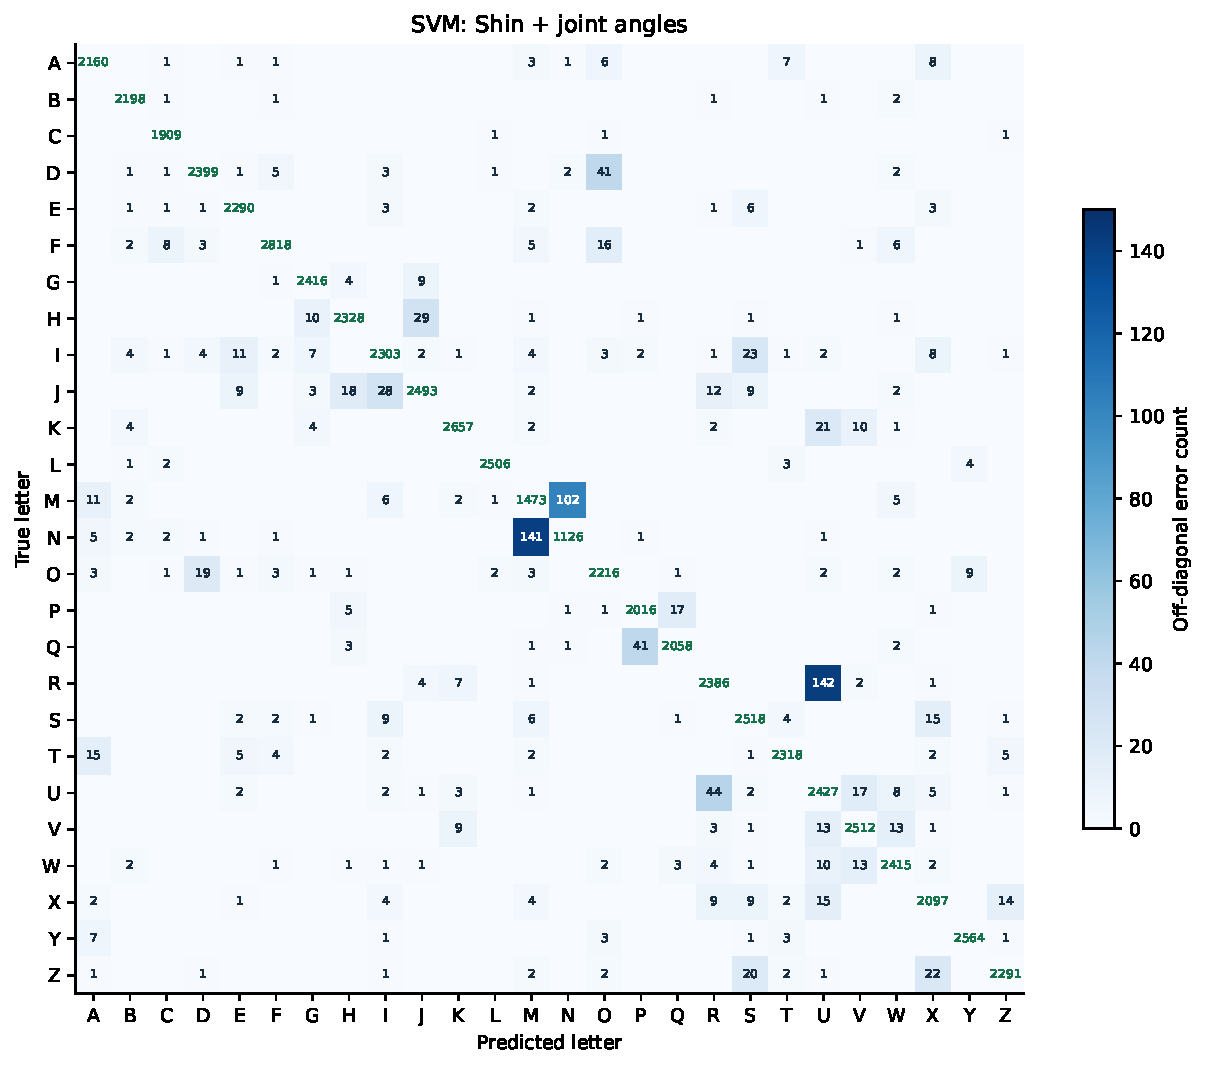
\includegraphics[width=.91\linewidth]{figures/confusion_angles.pdf}
\caption{Same images and folds with continuous angles added. Compare, for example, the M/N, R/U and D/O cells with the baseline matrix. Counts, rather than rounded percentages alone, expose small regressions.}\end{figure}
\clearpage
\section{Qualitative Examples and Feature Definitions}
\begin{figure}[h]\centering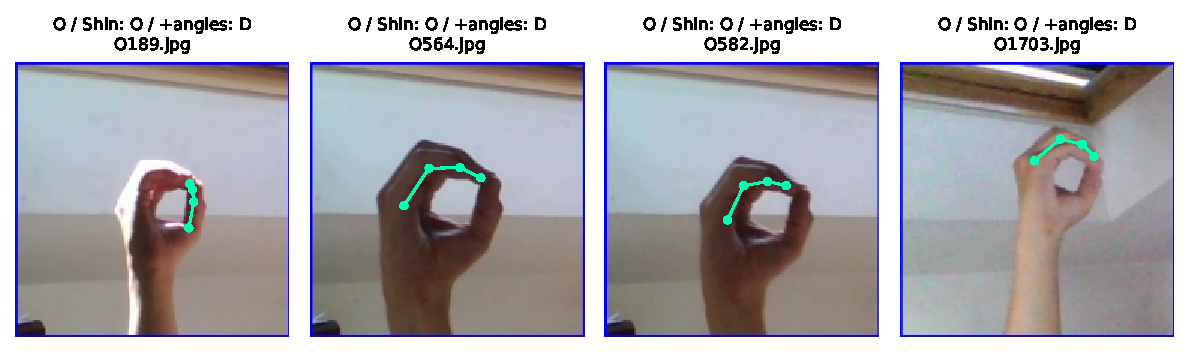
\includegraphics[width=\linewidth]{figures/o_errors.pdf}
\caption{Four actual Kaggle O images newly classified as D after adding angles; the index-finger landmarks are overlaid. These are static dataset errors, not recorded webcam rotation tests. Dataset labels are retained; no claim of manually revalidated signing correctness is made.}\end{figure}
\begin{figure}[h]\centering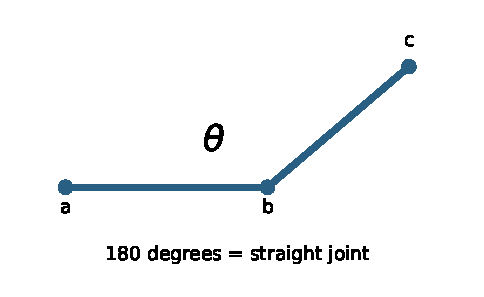
\includegraphics[width=.38\linewidth]{figures/angle.pdf}
\caption{Interior-angle convention for a joint centred at $b$. A straight joint approaches $180^\circ$; flexion reduces the angle.}\end{figure}
\begin{table}[h]\centering\caption{Landmark triplets for the 14 interior angles, using MediaPipe indices.}\begin{tabular}{lccc}\toprule
Finger & MCP & PIP & DIP / IP\\\midrule
Thumb & (1,2,3) & --- & IP: (2,3,4)\\
Index & (0,5,6) & (5,6,7) & (6,7,8)\\
Middle & (0,9,10) & (9,10,11) & (10,11,12)\\
Ring & (0,13,14) & (13,14,15) & (14,15,16)\\
Little & (0,17,18) & (17,18,19) & (18,19,20)\\\bottomrule\end{tabular}\end{table}
The fifteenth input is signed thumb-MCP deviation from the palm-oriented geometry implementation. The complete measured feature schema, unknown-state handling and thresholds are stored in \texttt{research/schema.py}, \texttt{research/geometry.py} and \texttt{config/thresholds.json}. The workbook parser preserves slash-separated alternatives as allowed sets. The user's workbook is unchanged; \texttt{config/proposal\_changes.json} contains the 49 proposed relaxations. They are applied in memory for the historical compatibility-score configuration, without retaining a second spreadsheet.

For U/V/K-style spread, fingers must be sufficiently separated and approximately coplanar; they need not be strictly parallel. Crossing detection uses a palm-oriented swap/depth proxy rather than assuming any two projected image lines prove a crossing. These engineering rules are auditable hypotheses and are not validated ground-truth annotations of anatomy.

\clearpage
\section{Paired Statistics and Weighting Details}\label{app:statistics}
Relative to the baseline, adding world-joint measurements fixes 143 formerly incorrect images and loses 76 formerly correct images, a net gain of 67. The descriptive accuracy change is 0.1112 percentage points. Six filename blocks give the changes below. Resampling these blocks with replacement 10,000 times (seed 42) gives a central 95\% sensitivity range of 0.0374--0.1947 percentage points. This is a descriptive stability check, not a valid independent-test confidence interval: there are only six non-person groups, possible cross-block correlation, overlapping training sets and exploratory model selection. We do not report a confirmatory $p$-value.
\begin{table}[h]\centering\caption{Paired world-joint-model changes by filename block.}\begin{tabular}{lrrr}\toprule
Block & Images & Net correct & Change (pp)\\\midrule
0000 & 10,504 & +4 & +0.0381\\
0001 & 11,399 & +27 & +0.2369\\
0002 & 12,101 & +2 & +0.0165\\
0003 & 12,255 & +5 & +0.0408\\
0004 & 10,009 & +23 & +0.2298\\
0005 & 3,983 & +6 & +0.1506\\\bottomrule\end{tabular}\end{table}

The primary weighting study evaluated 0.25/0.5/1/2 multipliers for continuous angles, categorical encodings and compatibility scores, with a single coordinate pass. In the targeted study, nested PIP weights were 2, 2, 0.5, 0.5 and 0.5 over the five outer folds. The selected MCP/PIP/DIP triples were (0.5,2,1), (1,2,0.5), (0.5,0.5,1), (2,0.5,1) and (1,0.5,1). These varying choices further caution against a universal rule that the index finger should receive higher weight.

\begin{table}[h]\centering\caption{Targeted SVM weighting on the 835-input angle configuration. Errors are directed true-label to prediction counts.}\begin{tabular}{lrrrr}\toprule
Configuration & Accuracy (\%) & Macro-F1 & O$\to$D & N$\to$M\\\midrule
Unweighted & 97.74776 & .975244 & 19 & 141\\
PIP weight 2 & 97.74941 & .975241 & 23 & 143\\
Nested PIP & 97.75273 & .975265 & 16 & 143\\
Nested MCP/PIP/DIP & 97.73946 & .975073 & 15 & 146\\\bottomrule\end{tabular}\end{table}

\section{Verification and Reproducibility}\label{app:verification}
The source repository retains one training dataset, the user's workbook, fixed thresholds and proposal changes, the compact standalone implementation, necessary study/live tools and tests, and compact measured evidence. Bulky model checkpoints, superseded datasets and obsolete interfaces are moved to a separate reversible archive; none is needed to interpret the reported tables. A central cached input matrix and sample/group metadata live inside the retained dataset directory. \texttt{REPRODUCE.md} documents setup, inventory validation, rebuilding descriptors from frozen landmarks, model comparisons, permutation analysis, ablations, tuning and report compilation.

The verification checks reconcile stored predictions with pooled accuracy, macro-F1, per-letter metrics and confusion totals; check one OOF prediction per image per model/variant; verify shared fold assignments and disjoint outer groups; and test feature widths, angle conventions, slash parsing, train-only preprocessing and index-weight application. Reconstructed descriptors are compared with the historical numeric cache. These checks support computational consistency; they do not validate source labels, estimated 3D anatomy or generalization to unseen signers. Large research experiments were completed before cleanup; refactoring preserves their numerical inputs and fixed profiles rather than silently reporting newly selected runs.

\section{Rubric Coverage and Outstanding Research}
\begin{tabular}{p{.20\linewidth}p{.72\linewidth}}\toprule
Rubric component & Coverage and limits\\\midrule
Abstract & Motivation, objective, methods, numerical outcomes and scope.\\
Introduction & Field, motivation, contribution, questions and structure.\\
Related work & Baseline geometry, landmark estimation, alternative sensing/classification, permutation reliance and selection bias.\\
Methods & Representations, angle equation, model objectives, weighting and preprocessing.\\
Experiments/analysis & Matched baseline, dataset filtering, ablations, two algorithms, nested weighting, per-letter errors and descriptive paired analysis. No untouched final test or confirmatory significance claim.\\
Discussion & Meaning, strengths, limitations, ethics and AI-generation disclosure.\\
Conclusions & Modest observed angle benefit and prospective person/viewpoint-separated evaluation.\\\bottomrule\end{tabular}

The main report now answers the explicit-feature comparison question through RQ1--RQ3. Later webcam experiments are supporting diagnostics, not unfinished conditions for that answer. A prospective signer-separated evaluation and independent review of the workbook remain valuable follow-ups. The detailed rubric assessment is retained separately in \texttt{paper/RUBRIC\_REVIEW.md}.

\clearpage
\section{Technical Method Details}
\subsection{Landmarks and Baseline}
Images are processed with MediaPipe Hand Landmarker. The intended extraction settings are IMAGE mode, up to two hands, and detection/presence thresholds of 0.5; only exactly one accepted hand is used. Historical records contain the MediaPipe version and landmarks, but not the threshold values. Thus default-setting provenance cannot be independently confirmed for the historical cache. We preserve these landmarks for all comparisons rather than rerun detection differently per model.

The Shin implementation follows the paper's pair list: 190 pairwise distance features and 630 axis-direction features, for 820 features overall. Distance features are normalized per image; direction features are cosine-based encodings of inter-landmark vectors relative to axes. The local implementation preserves the paper's listed pair exclusions. Features use image landmarks for the baseline and estimated world landmarks for the added hand geometry.

\begin{figure}[t]
\centering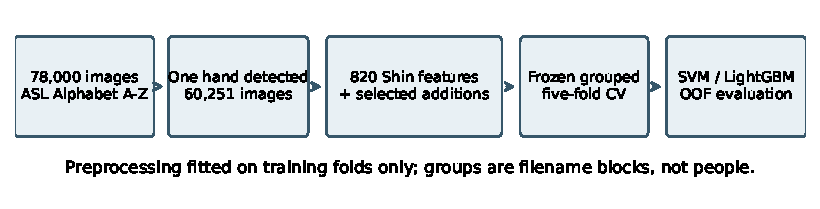
\includegraphics[width=\linewidth]{figures/pipeline.pdf}
\caption{Evaluation pipeline. Every compared model uses the same 60,251 accepted images and frozen outer folds. Detection coverage and conditional classification accuracy are separate quantities.}
\label{fig:pipeline}
\end{figure}

\subsection{Interpretable Additions}
For consecutive landmarks $a,b,c$, an interior bending angle is
\begin{equation}
\theta(a,b,c)=\arccos\frac{(a-b)^\top(c-b)}{\|a-b\|\,\|c-b\|}\frac{180}{\pi}.
\end{equation}
A straight joint approaches $180^\circ$. We use thumb MCP/IP and MCP/PIP/DIP for the other four fingers: 14 interior angles. A signed thumb-MCP deviation adds a fifteenth measurement. MCP measurements are landmark-based proxies, not calibrated clinical joint measurements. The retained phrase ``angles'' below always means all 15 additions, not a fourteenth-angle-only experiment.

Categorical features encode bent, partly bent and extended joints; a binary B-shaped/non-B-shaped thumb MCP; and spread, suspected crossing and thumb contact relations. An unknown state is retained. Thresholds are fixed across folds. Non-thumb flexion uses $\leq130^\circ$ for bent and $\geq150^\circ$ for extended, with intermediate values partly bent. Finger spread requires separation in approximately the same plane; splaying is allowed. Crossing and contact are geometric proxies and remain sensitive to occlusion and depth estimates.

The workbook gives the allowed categories for each letter. A slash means a set of acceptable alternatives, not a new combined class. One-hot measured categories yield 70 inputs. For each candidate letter $\ell$, a compatibility score averages the proportion of specified workbook cells whose allowed set contains the measured category. This produces 26 scores. All 26 are computed for every image without accessing its true label. A fixed 49-cell slash-relaxation proposal was developed in earlier exploratory work; its changes are preserved separately from the user's original workbook. This reference design was not nested within the later evaluation.

\subsection{Models, Scaling and Weighting}
The primary SVM uses an RBF kernel, $C=10$, \texttt{gamma=scale} and balanced class weights. This differs from the paper-profile $C=1000$ with no class balancing. Its soft-margin objective balances margin size against weighted classification slack. For input blocks $z_b$ and weights $w_b$, the RBF similarity is
\begin{equation}
K(x,x')=\exp\!\left(-\gamma\sum_b w_b^2\|z_b(x)-z_b(x')\|^2\right).
\end{equation}
For each binary letter pair, the kernel SVM minimizes the regularized hinge loss
\[
\frac12\|w\|^2+C\sum_i\omega_i\max(0,1-y_i(w^\top\phi(x_i)+b)),
\]
where $y_i\in\{-1,1\}$, $\phi$ is the kernel feature mapping and $\omega_i$ combines class and sample weights. The multiclass decision uses pairwise voting. LightGBM instead optimizes multiclass log loss with tree-complexity control. These objectives were not modified to prefer individual letters.

Thus a multiplier of two contributes a factor of four inside the squared distance, while \texttt{gamma=scale} also changes with the input variance. Angle median imputation and standardization are fitted within each training fold; baseline descriptors and categorical/compatibility values pass through unchanged. No missing angles occurred in the retained cache.

LightGBM optimizes multiclass log loss through boosted trees, using 100 estimators, 31 leaves, learning rate 0.1 and minimum child size 20. Its fixed project profile is not a replication of the paper's tuned LightGBM settings. Group weighting searches use inner-fold macro-F1, breaking ties by accuracy. They make one coordinate pass, not an exhaustive global search.


\section{Earlier Experimental Settings and Results}
\subsection{Implementation and Experimental Sequence}
Experiments use Python 3.12, MediaPipe 0.10.35, scikit-learn 1.8.0 and LightGBM 4.7.0. An earlier three-fold pilot tested 81 continuous/binary finger-geometry descriptors, alone and combined with baseline descriptors. This differs from the later 70-column categorical encoding and is not mixed into the five-fold table. The pilot feature-only model reached 93.71\% mean fold accuracy, versus 97.43\% for the baseline; combining them did not improve the baseline. It did not isolate replacement of only the 190 distances while retaining all 630 directions.

The main sequence compares the 820 baseline, all 111 additions (931 total), then isolated angle and compatibility-score additions. Grouped permutation analysis shuffles whole related columns jointly on held-out data, five repeats with at most 100 images per letter per fold. Ablations remove a block and refit. These analyses share the fixed full-input model and should not be interpreted as interchangeable measures.

Block weighting tries 0.25, 0.5, 1 and 2. Targeted index MCP/PIP/DIP weighting tries 0.5, 1 and 2. Both use five outer and three inner group folds, with inner training and validation capped at 150 images per letter for cost. The final outer fits use all outer-training images. This is bounded exploratory tuning, not exhaustive hyperparameter optimization.


\subsection{Isolated SVM and LightGBM results}
\begin{table}[h]\centering\caption{Detailed original isolated comparison; these results concern matched accepted images.}
\begin{tabular}{lrrrrr}\toprule
Representation & Inputs & SVM acc. (\%) & SVM macro-F1 & LGBM acc. (\%) & LGBM macro-F1\\\midrule
\tableinput result_rows.tex
\bottomrule\end{tabular}\end{table}

The full 931-input SVM scored 97.62826\% and LightGBM 97.16353\%. Removing categorical one-hot columns produced 97.74444\% for SVM, matching the isolated angle-plus-workbook model. In the grouped permutation analysis, shuffling angles reduced SVM macro-F1 by 0.570 percentage points, compared with 0.049 for categories and 0.008 for workbook compatibility scores. For LightGBM these drops were 0.031 and 0.200 for angles and compatibility scores. These overlapping reliance measures are not additive or causal.

The source article reports 87.60\% ASL Alphabet combined-feature SVM accuracy, no matching F1 metric, and a held-out evaluation with tuning rather than this filtered grouped protocol. It also states 780,000 images inconsistently with 26 times 3,000; the actual inventory is 78,000. The local paper-profile SVM ($C=1000$, no balancing) reached 97.66145\%; changing this setting alone does not reconcile the protocols. Detection, data selection and split differences have not been isolated experimentally.


\section{Tilt Augmentation and Recorded Development Study}
The original training input contains 820 Shin values plus 15 angles. For each of the 210 unit direction vectors $d_{ij}$, the augmentation uses
\[
R_x(\alpha)=\begin{bmatrix}1&0&0\\0&\cos\alpha&-\sin\alpha\\0&\sin\alpha&\cos\alpha\end{bmatrix},
\qquad d'_{ij}=R_x(\alpha)d_{ij},\qquad \alpha\in\{-15^\circ,0,15^\circ\}.
\]
Only input columns 190--819 change (zero-based indexing). The first 190 normalized distances and final 15 intrinsic measurements stay fixed. This rotation is performed in normalized landmark-feature coordinates and is an approximation, not a full physical wrist or perspective model. It does not simulate occlusions or detector errors.

The all-letter run uses 180,753 fitting rows from 60,251 originals, with weight $1/3$ per row. Class balancing and gamma=scale are applied through the fixed SVM pipeline. The C-only run adds two copies of each of the 1,912 C originals, producing 64,075 fitting rows; 58,339 other images remain single examples. Each C source retains total sample weight one, and other rows have weight one. For selective augmentation, preprocessing, balanced class weights and the resolved gamma value are fitted on original fitting rows, avoiding unintended class-frequency or scaling changes. The C-only full-data resolved gamma and class weights match the baseline exactly. The earlier all-letter run computed gamma over its augmented matrix, so the three-way comparison is not a strict single-factor ablation of that numeric parameter.

Both variants were tested on the same original five grouped folds. Augmentation occurs only after splitting, inside the fitting partition. Each variant yields 60,251 original validation predictions. The all-letter variant recovers 57 errors and loses 84 correct predictions: 58,867 correct versus 58,894 for the angle baseline. Its accuracy is 97.70294269\% and macro-F1 0.974685870. The C-only variant has the same 58,894 correct images as baseline, with zero recoveries or losses and three wrong-to-wrong label changes; macro-F1 changes from 0.975243912 to 0.975244649. This difference is practically negligible.

The guided development session contains 27 planned captures: C/D/O, three qualitative wrist positions and three repetitions. The intended label and step are fixed; predictions are hidden during collection. All 27 have accepted detections. The session predates candidate fitting and never enters training. The reference Shin-only full-data fit scores 17/27 and C/D/O macro-F1 0.609524; the joint-angle fit scores 17/27 and 0.610035. All-letter tilt scores 18/27 and 0.642439; C-only tilt returns the same predictions as the joint-angle baseline. Joint-angle-model counts by intended letter are C=3/9, D=8/9, O=6/9; all-letter tilt changes only the number correct for O to 7/9. One wrong C prediction also changes from D to O, lowering O precision while improving its recall.

These are development outcomes, not independent test results. The reserved evaluation directory contained zero completed captures when these experiments were run. The previously inspected second-person O example is an exploratory illustration and is not added to the primary 27. No angle/axis search was conducted within either augmentation run, but the research sequence as a whole is exploratory.

The main input/model/image hashes and saved predictions were audited. In the 28 records comprising the development round and extra O example, all image hashes matched and all 835 feature vectors and predictions were reconstructed. The additional reference model is fitted on the same 60,251 original images using only 820 inputs; its live-bundle schema is distinguished from the 835-input models. Snapshot exports retain the selected model's hash, input variant and matching feature width.

Reproduction commands, evidence paths and the live model-label mapping are documented in \texttt{REPRODUCE.md}.
\clearpage
\section{Later Webcam and Representation Diagnostics}
These experiments followed the primary feature comparison. They are retained for transparency and hypothesis generation; they do not expand the main report's research question into a claim that webcam or viewpoint problems have been solved. Stored development errors were reused to motivate successive changes, so their outcomes are not independent final-test evidence.

\subsection{Larger G/H Rotations and Projected Angles}
A selective G/H augmentation rotates only the 630 image-axis direction values around the camera-$y$ axis by $-90^\circ$, $90^\circ$ and $180^\circ$, retaining each original. There are 4,801 G/H originals and 74,654 fitting rows overall. Each selected source contributes four rows of weight 0.25; other classes occur once with weight one. Preprocessing, balanced class weights and resolved gamma are determined on the original fitting partition. This is a numerical landmark-feature rotation, not a realistic palm/back-of-hand rendering or occlusion simulation.

A separate unaugmented candidate adds 14 internal angles measured from projected image landmarks, after converting normalized $x,y$ into pixels with the detector image width and height. It has 849 inputs: the original 820, 15 estimated 3D measurements and 14 projected angles. The same function is used for training and live inference. Median imputation and standard scaling of all 29 angle inputs are fitted only on each fitting partition. Camera captures are not used for fitting either candidate.

\begin{table}[h]\centering\caption{Supporting 26-class experiments using the same frozen five folds. These extend the research sequence beyond the main feature comparison.}
\begin{tabular}{lrrr}\toprule
Model & Correct / 60,251 & Accuracy (\%) & Macro-F1\\\midrule
Shin + 3D measurements & 58,894 & 97.74776 & .97524391\\
Selective G/H rotation & 58,888 & 97.73780 & .97516874\\
Shin + 3D + projected angles & 58,861 & 97.69298 & .97465145\\\bottomrule\end{tabular}\end{table}

Selective G/H rotation fixes nine formerly wrong predictions and loses 15 correct ones. The projected-angle model fixes 70 and loses 103. Its five-fold accuracy declines in four folds and improves in one. Neither is an overall improvement on the 835-input reference. On the 27 earlier C/D/O development captures, the projected-angle model returns 16 correct versus 17 for the angle baseline.

The selected GH-handrug development round contains 11 errors from the G/H-rotation model: G$\to$H, C$\to$D, F$\to$B, K$\to$H, N$\to$M, O$\to$D, P$\to$H, S$\to$E, T$\to$L, X$\to$H and Y$\to$A. Replaying the original 835-input model on these same landmarks recovers K and X; adding projected angles also recovers T. The newest G remains misclassified. This is a selected-error replay, not a representative live-accuracy comparison.

\subsection{G/H-Only Diagnostic Classifiers}
The primary 26-class angle SVM recognizes 2,416/2,430 accepted G images correctly (99.424\% recall). Its 14 true-G errors are nine J, four H and one F. For H, 2,328/2,371 are correct (98.186\%); ten are G and 29 J, with four other errors. Thus strong accepted-image dataset recognition coexists with the recorded webcam failures.

Three fixed binary SVMs were fitted using only 3D angles, only projected angles or both. The same frozen folds were restricted to their 4,801 G/H images. Every variant used training-only median imputation and standard scaling, with RBF $C=10$, balanced classes and gamma=scale. They are easier two-label tasks with different inputs, not replacements for the 26-class recognizer.

\begin{table}[h]\centering\caption{Binary G/H diagnostics. The fourth row is an explicitly post-hoc, targeted ablation after inspecting the first three.}
\begin{tabular}{lrrr}\toprule
Inputs & Number & Accuracy (\%) & Macro-F1\\\midrule
3D measurements & 15 & 96.563 & .96563\\
Projected 2D angles & 14 & 95.793 & .95791\\
Both representations & 29 & 96.584 & .96584\\
Middle PIP only, 3D + 2D & 2 & 94.085 & .94084\\\bottomrule\end{tabular}\end{table}

All three fuller binary variants still classify the newest selected G as H. Its middle-PIP estimate is $95.3^\circ$, near the training-G median $86.7^\circ$ and below the H median $166.2^\circ$. Other measurements disagree with typical G: the index PIP is $134.9^\circ$ against a G median $172.6^\circ$, while middle DIP is $161.0^\circ$ against medians $113.2^\circ$ for G and $170.4^\circ$ for H. Its signed thumb deviation is $-1.5^\circ$ against medians around $36$--$37^\circ$ for both. The classifier sees a combination, not just a count of straight fingers.

The two-input middle-PIP ablation recovers the two selected G examples and one H example, but has lower grouped dataset performance. It was proposed after inspecting these known failures and is exploratory. A later selected H with visible palm is called G by all six 26-class variants, although its estimated index/middle PIP angles are $165.5^\circ$/$159.8^\circ$. The binary diagnostics call it H. This counterexample shows that palm versus back-of-hand viewpoint alone cannot explain every recorded error.

A four-view protocol for three participants (G/H, palm, oblique palm, oblique back-of-hand, back-of-hand; five repetitions) has been implemented, but no completed cohort evaluation is claimed here. The qualitative views are not calibrated physical angles. New balanced and signer-separated observations would be needed for a prospective viewpoint comparison.

Evidence and reproduction commands are in \texttt{results/rotation\_GH\_01/}, \texttt{results/angles\_2d\_01/}, \texttt{results/gh\_classifier\_01/}, \texttt{results/gh\_middle\_01/} and \texttt{REPRODUCE.md}. Saved image/model hashes, raw measurements and predictions support computational replay, not anatomical or linguistic ground truth.

\clearpage
\section{Exploratory preprocessing experiments for RQ2}
\label{app:rq2-pilot}

\subsection{Provenance and purpose}
The initial baseline, N47 probes and letter-balanced pilot were implemented and executed by the Codex assistant using the local Kaggle ASL Alphabet images. The student subsequently reported executing the three-stage workflow. The completed \texttt{test\_110} exports support the reproduction documented at the end of this appendix. Program outputs establish the recorded outcomes; operator identity is based on the student's report. Visual assessment remains outstanding.

RQ2 concerns recovery of visually plausible hand landmarks among initially missed images. The measurements below establish technical recovery. The visual plausibility of all recovered configurations has yet to be assessed using a fixed rubric. N47 and other inspected pilot images should be identified as development data when constructing a subsequent evaluation set.

\subsection{Fresh baseline and training}
The baseline processed 78,000 original A--Z training images, comprising 3,000 images per letter. The additional classes were excluded. MediaPipe Hand Landmarker 0.10.35 ran in IMAGE mode, with a maximum of two hands and detection and presence thresholds both set to 0.50. The model file was \texttt{models/hand\_landmarker.task}. A result received \texttt{ok} when exactly one hand was returned and the project's geometric validation passed.

\begin{table}[ht]\centering
\caption{Fresh detection outcomes on original A--Z training images.}
\label{tab:rq2-baseline}
\begin{tabular}{lrr}\toprule
Outcome & Images & Percentage\\\midrule
One valid hand (\texttt{ok}) & 60,251 & 77.245\\
Zero hands (\texttt{no\_hand}) & 17,598 & 22.562\\
Multiple hands & 151 & 0.194\\
Invalid geometry & 0 & 0.000\\\midrule
Total & 78,000 & 100.000\\\bottomrule
\end{tabular}
\end{table}

A fresh SVM letter classifier was fitted to the 60,251 accepted images using 820 Shin descriptors and 15 angle features. This produced \texttt{runs/clean\_training/asl\_clean.joblib}. Its fit has no independent test score. The recovery experiments below use the pretrained MediaPipe detector; the letter classifier does not determine whether a hand is detected.

\subsection{N47 development example}
The original N47 image returned \texttt{no\_hand}. One application of dilation with a square \(3\times3\) kernel changed its output to \texttt{ok} at the same detector thresholds. Erosion and the tested Canny overlay retained \texttt{no\_hand}. In separate threshold probes on the original pixels, lowering only the detection threshold to 0.49 retained \texttt{no\_hand}, while 0.45 yielded \texttt{ok}. These probes show sensitivity to both preprocessing and threshold choice.

The initial N47 probes were executed as terminal commands, and their outputs were recorded in the conversation. They were not exported as a dedicated CSV. The original-versus-dilation transition was subsequently rerun when generating the example images below. The exact internal detection score was not recorded.

\begin{figure}[ht]\centering
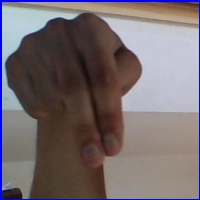
\includegraphics[height=30mm]{rq2_examples/N47_original.png}\hspace{8mm}
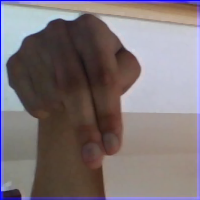
\includegraphics[height=30mm]{rq2_examples/N47_dilated.png}\hspace{8mm}
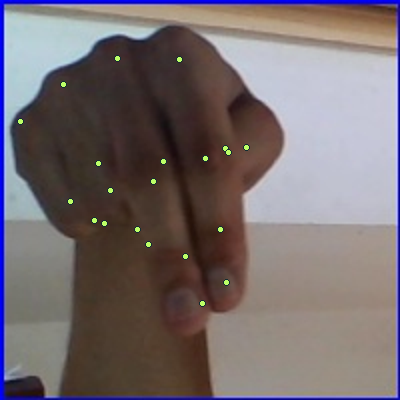
\includegraphics[height=30mm]{rq2_examples/N47_overlay.png}
\caption{N47 in its original form (left), after dilation (centre), and with recovered points overlaid on the original pixels (right). The overlay supports inspection; it does not constitute an independent landmark accuracy assessment.}
\label{fig:rq2-n47}
\end{figure}

\clearpage
\subsection{Letter-balanced pilot}
Using random seed 42, the pilot selected 20 initially missed and 10 initially accepted images per letter, giving 520 misses and 260 controls. The original status was rechecked before applying each transformation. Every selected photo received each of the three transformations below, with fixed detector settings.

\begin{itemize}
\item Dilation used \texttt{cv2.dilate} with a \(3\times3\) square kernel and one iteration.
\item Erosion used \texttt{cv2.erode} with the same kernel and iteration count.
\item The Canny overlay used a grayscale conversion, a \(5\times5\) Gaussian blur and Canny thresholds of 50 and 150. The three-channel edge map was added to the original RGB image with weights 0.25 and 1.0, respectively.
\end{itemize}

Image dimensions were retained, and processed arrays were supplied directly to the detector. Technical recovery means a transition from \texttt{no\_hand} to \texttt{ok}. Control loss means that an originally accepted image no longer received \texttt{ok}.

\begin{table}[ht]\centering
\caption{Exploratory pilot outcomes. Recovery denominators are 520 misses; loss denominators are 260 controls.}
\label{tab:rq2-pilot}
\begin{tabular}{lrrrr}\toprule
Transformation & Recovered & Recovery (\%) & Control losses & Loss (\%)\\\midrule
Dilation & 130 & 25.00 & 6 & 2.31\\
Erosion & 64 & 12.31 & 8 & 3.08\\
Canny overlay & 49 & 9.42 & 28 & 10.77\\\bottomrule
\end{tabular}
\end{table}

The pilot gave equal weight to each letter, whereas the complete set of missed images has unequal letter counts. Its recovery percentage therefore does not directly estimate recovery across all 17,598 misses. Control losses describe applying preprocessing to already accepted images. A second-attempt procedure restricted to baseline misses bypasses these controls.

\subsection{Code and retained evidence}
All paths below are relative to the project root containing \texttt{app.py}.
\begin{itemize}
\item \texttt{research/data.py}, class \texttt{Detector}, defines detector settings and geometric validation.
\item \texttt{research/clean\_training.py} runs the baseline and prepares accepted inputs. The fresh classifier fit uses \texttt{--fresh-fit} in \texttt{research/live\_model.py}.
\item \texttt{research/morphology\_pilot.py} contains the transformations, deterministic sampling, paired comparisons and pilot exports.
\item \texttt{runs/clean\_training/all\_images.csv}, \texttt{no\_hand.csv} and \texttt{by\_letter.csv} contain the baseline inventory and summaries.
\item The pilot directory is \texttt{runs/clean\_training/morphology\_pilot/}. It contains \texttt{per\_foto.csv} with paired outcomes, \texttt{summary.csv} with aggregate results and \texttt{controle\_*.jpg} with overlays of recovered detections.
\end{itemize}

The original pilot exports status changes and rendered overlays. The subsequent three-stage workflow also exports landmark coordinates in \texttt{retry\_landmarks.jsonl}. A completed visual-review dataset remains outstanding. The earlier \texttt{historical\_image\_audit.py} reconstructed historical cohort membership. The fresh detector outputs listed above support the present baseline counts.

\subsection{Reproduction and next measurement}
Run \texttt{python -m research.clean\_training --out runs/clean\_training}
from the project root with the configured Python environment. The command requires a new output directory. The existing baseline can be used to rerun \texttt{python -m research.morphology\_pilot}; this command writes to the existing pilot output paths. Preserve the original evidence before rerunning it.

\clearpage
\subsection{Student-reported reproduction and program evidence}
\label{app:rq2-reproduction}
The completed run is \path{experiments/hand_detection_recovery/runs/test_110}.
It used \texttt{--limit 110}, selecting A1--A110 in dataset order. This is a technical reproduction on a single letter. It contains no N47 image and does not estimate recovery across A--Z.
The preserved evidence is located at \path{paper/evidence/rq2_test_110}.
The following tables were checked against the paired rows and landmark exports, in addition to the program summary.

\begin{table}[ht]\centering
\caption{Recomputed outcomes for \texttt{test\_110}. Recovery rates use 46 baseline misses as the denominator.}
\begin{tabular}{lrr}\toprule
Quantity & Count & Percentage\\\midrule
Original images & 110 & 100.00\\
Originally accepted & 64 & 58.18\\
Initially missed & 46 & 41.82\\\midrule
Recovered by dilation & 6 & 13.04\\
Recovered by erosion & 2 & 4.35\\
Recovered by Canny overlay & 0 & 0.00\\
Recovered by at least one variant & 8 & 17.39\\\bottomrule
\end{tabular}
\end{table}

Counting each image once, original acceptance plus any technically successful retry gives \(72/110=65.45\%\) coverage, compared with \(64/110=58.18\%\) initially. The increase is 7.27 percentage points. This combined outcome allows any of the three variants to succeed.

\begin{table}[ht]\centering
\caption{Recovered images from \texttt{per\_image.csv}. All originally had status \texttt{no\_hand}.}
\begin{tabular}{ll}\toprule
Successful variant & Original filenames\\\midrule
Dilation & A59.jpg, A74.jpg, A75.jpg, A90.jpg, A92.jpg, A98.jpg\\
Erosion & A85.jpg, A89.jpg\\\bottomrule
\end{tabular}
\end{table}

\paragraph{Evidence traceability.}
\texttt{baseline.csv} records original detections. \texttt{no\_hand.csv} identifies the 46 candidates.
\texttt{processed.csv} maps their 138 variant images to original IDs and records image checksums.
\texttt{per\_image.csv} supplies paired statuses and successful variants.
\texttt{summary.csv} gives aggregate counts, while \texttt{unrecovered.csv} identifies the 38 remaining misses.
\texttt{retry\_landmarks.jsonl} contains the retry outputs and recovered coordinates.
\texttt{settings.json} records MediaPipe 0.10.35, OpenCV 4.14.0, filter parameters, detector settings and code/model hashes.
The archive's \texttt{evidence\_manifest.json} records SHA256 checksums of these exports.
Absolute image paths refer to the original workstation; the PNGs remain in the source run.

\paragraph{Reproduction.}
Use the project's configured Python environment from the root containing \texttt{app.py}.
The following command invokes the existing baseline, preprocessing and retry functions in sequence:
\begin{verbatim}
python experiments/hand_detection_recovery/run.py --name test_110 --limit 110
\end{verbatim}
The wrapper starts clean and deletes existing outputs with that run name. Use a new name to preserve a live run, or add \texttt{--resume} to continue it. The separate evidence archive survives cleaning the run folder.

\paragraph{Verification of exported results.}
The read-only check below recomputes recovery counts and percentages, checks image-ID and variant correspondence, and confirms that accepted retry records contain one hand with 21 image landmarks.
\begin{verbatim}
python experiments/hand_detection_recovery/verify_results.py \
  --run paper/evidence/rq2_test_110
\end{verbatim}
Enter this as one line in PowerShell, omitting the displayed backslash.
Verification passed for the archived exports. This establishes internal consistency of the recorded measurements. Visual landmark quality and the final dataset-wide recovery result remain to be evaluated. At inspection, \texttt{full\_dataset\_01} contained partial progress but no completed result summary.


\end{document}

